\section{中性子輸送}

\subsection{中性子輸送の位置づけ}
原子炉物理が原子炉内の中性子の挙動と原子核の反応を予測する学問であるとすれば、中性子輸送は
その中核をなす部分である。中性子の挙動は中性子輸送そのものであるし、原子核の反応を予測するには
中性子の分布を知ることが必須である。原子核の反応を正確に予測することができれば、核燃料の燃焼が
進んだ時の炉心を予測でき、更に先の炉心の状態を精度よく予測していくことができる。

ある核種$i$について炉心内での量(数密度$N_i$)の増減を予測するには、生成・消滅に関する次の方程式を解けばよい。
\begin{align}
  \frac{dN_i}{dt} &= (\text{生成率}) + (\text{変換率}) + (\text{消滅率}) \notag \\
  &= 
%  \sum_j \gamma_{ji} \sigma_{f,j} N_j \phi 
%  + \sigma_{c,i-1} N_{i-1} \phi 
%  + \sum_k \lambda_k N_k \notag \\
%  &\quad - \sigma_{a,i} N_i \phi 
%  - \lambda_i N_i \notag \\
  \begin{aligned}
    &\underbrace{\sum_j \gamma_{ji} \sigma_{f,j} N_j \phi}_{\text{核種$j$の\emph{核分裂による生成の総和}}} 
    + \underbrace{\sigma_{c,i-1} N_{i-1} \phi}_{\text{核種$i-1$の\emph{捕獲による生成}}} \\
    &+ \underbrace{\sum_k \lambda_k N_k}_{\text{核種$k$の\emph{崩壊による生成の総和}}} 
    - \underbrace{\sigma_{a,i} N_i \phi}_{\text{核種$i$の\emph{吸収による変換}}} 
    - \underbrace{\lambda_i N_i}_{\text{核種$i$の\emph{崩壊による消滅}}}
  \end{aligned}
  \label{BurnupEq}
\end{align}

この式~\eqref{BurnupEq}は\emph{燃焼方程式}と呼ばれる連立の一階常微分方程式である。
全ての核種の数密度をベクトルとして見ると、この式は
\begin{align}
  \frac{d\vec{N}}{dt} = \bm{A} \vec{N}  \label{BurnupEq2}
\end{align}
と表記できる。この$\bm{A}$は「燃焼マトリックス」と呼ばれる行列である。
燃焼マトリックス内の各反応率が全て一定であれば、
式~\eqref{BurnupEq2}の解析解は
\begin{align}
  \vec{N}(t) = \vec{N}(0) \exp{ (\bm{A} t) } \label{BurnupEqAnlSol}
\end{align}
である。ところが、数密度は位置によって異なるはずなので、ここで求まる$\vec{N}(t)$は「\emph{ある位置}、
ある時刻の核種数密度$\vec{N}(\bm{r},t)$」とすべきであるし、燃焼マトリックスについても
中に出てくる$\phi$が、「\emph{ある位置、ある時刻}の中性子束$\phi(\bm{r},t)$」であるため、
反応率は位置や時間によって変化する。したがって、実際の原子炉の解析では時間的・空間的な
\emph{離散化}を施すことになる。
\begin{figure}[htbp]
  \begin{center}
  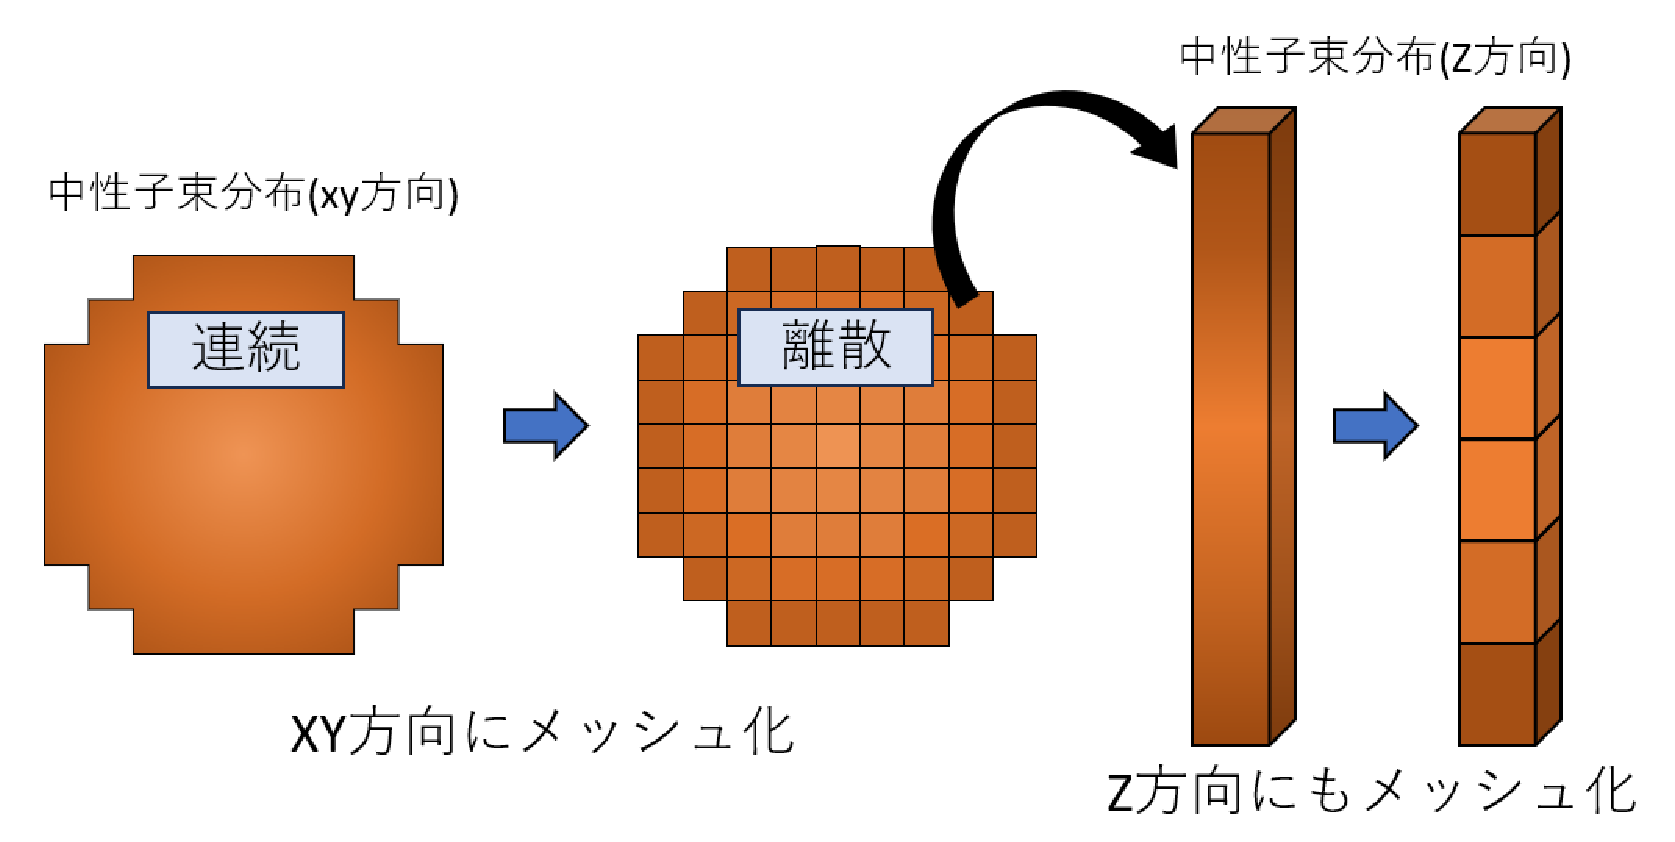
\includegraphics[width=120mm]{figure/discretization.eps}
  \caption{炉心の中性子束分布をメッシュ化して空間的に離散化する}\label{discretization}
  \end{center}
\end{figure}
Fig.~\ref{discretization}、Fig.~\ref{time-discretization}はPWRや高速炉の
炉心計算の離散化例である。XYZ方向に区切られたメッシュ内で、中性子束や燃料組成を
均一とする空間的離散化を適用し、計算条件として与えている。
時間については、\emph{燃焼サイクルを複数のステップに区切り、その期間内の反応率
が一定であるとみなし}離散化している。各燃焼ステップごとに中性子束分布は
変化するため、ステップ毎に中性子束分布を計算し、ステップ後の燃料組成を
求める必要がある。故に中性子束分布計算と燃焼計算を反復する必要があり、
計算の誤差は繰り返し毎に蓄積する。

\begin{figure}[htbp]
  \begin{center}
  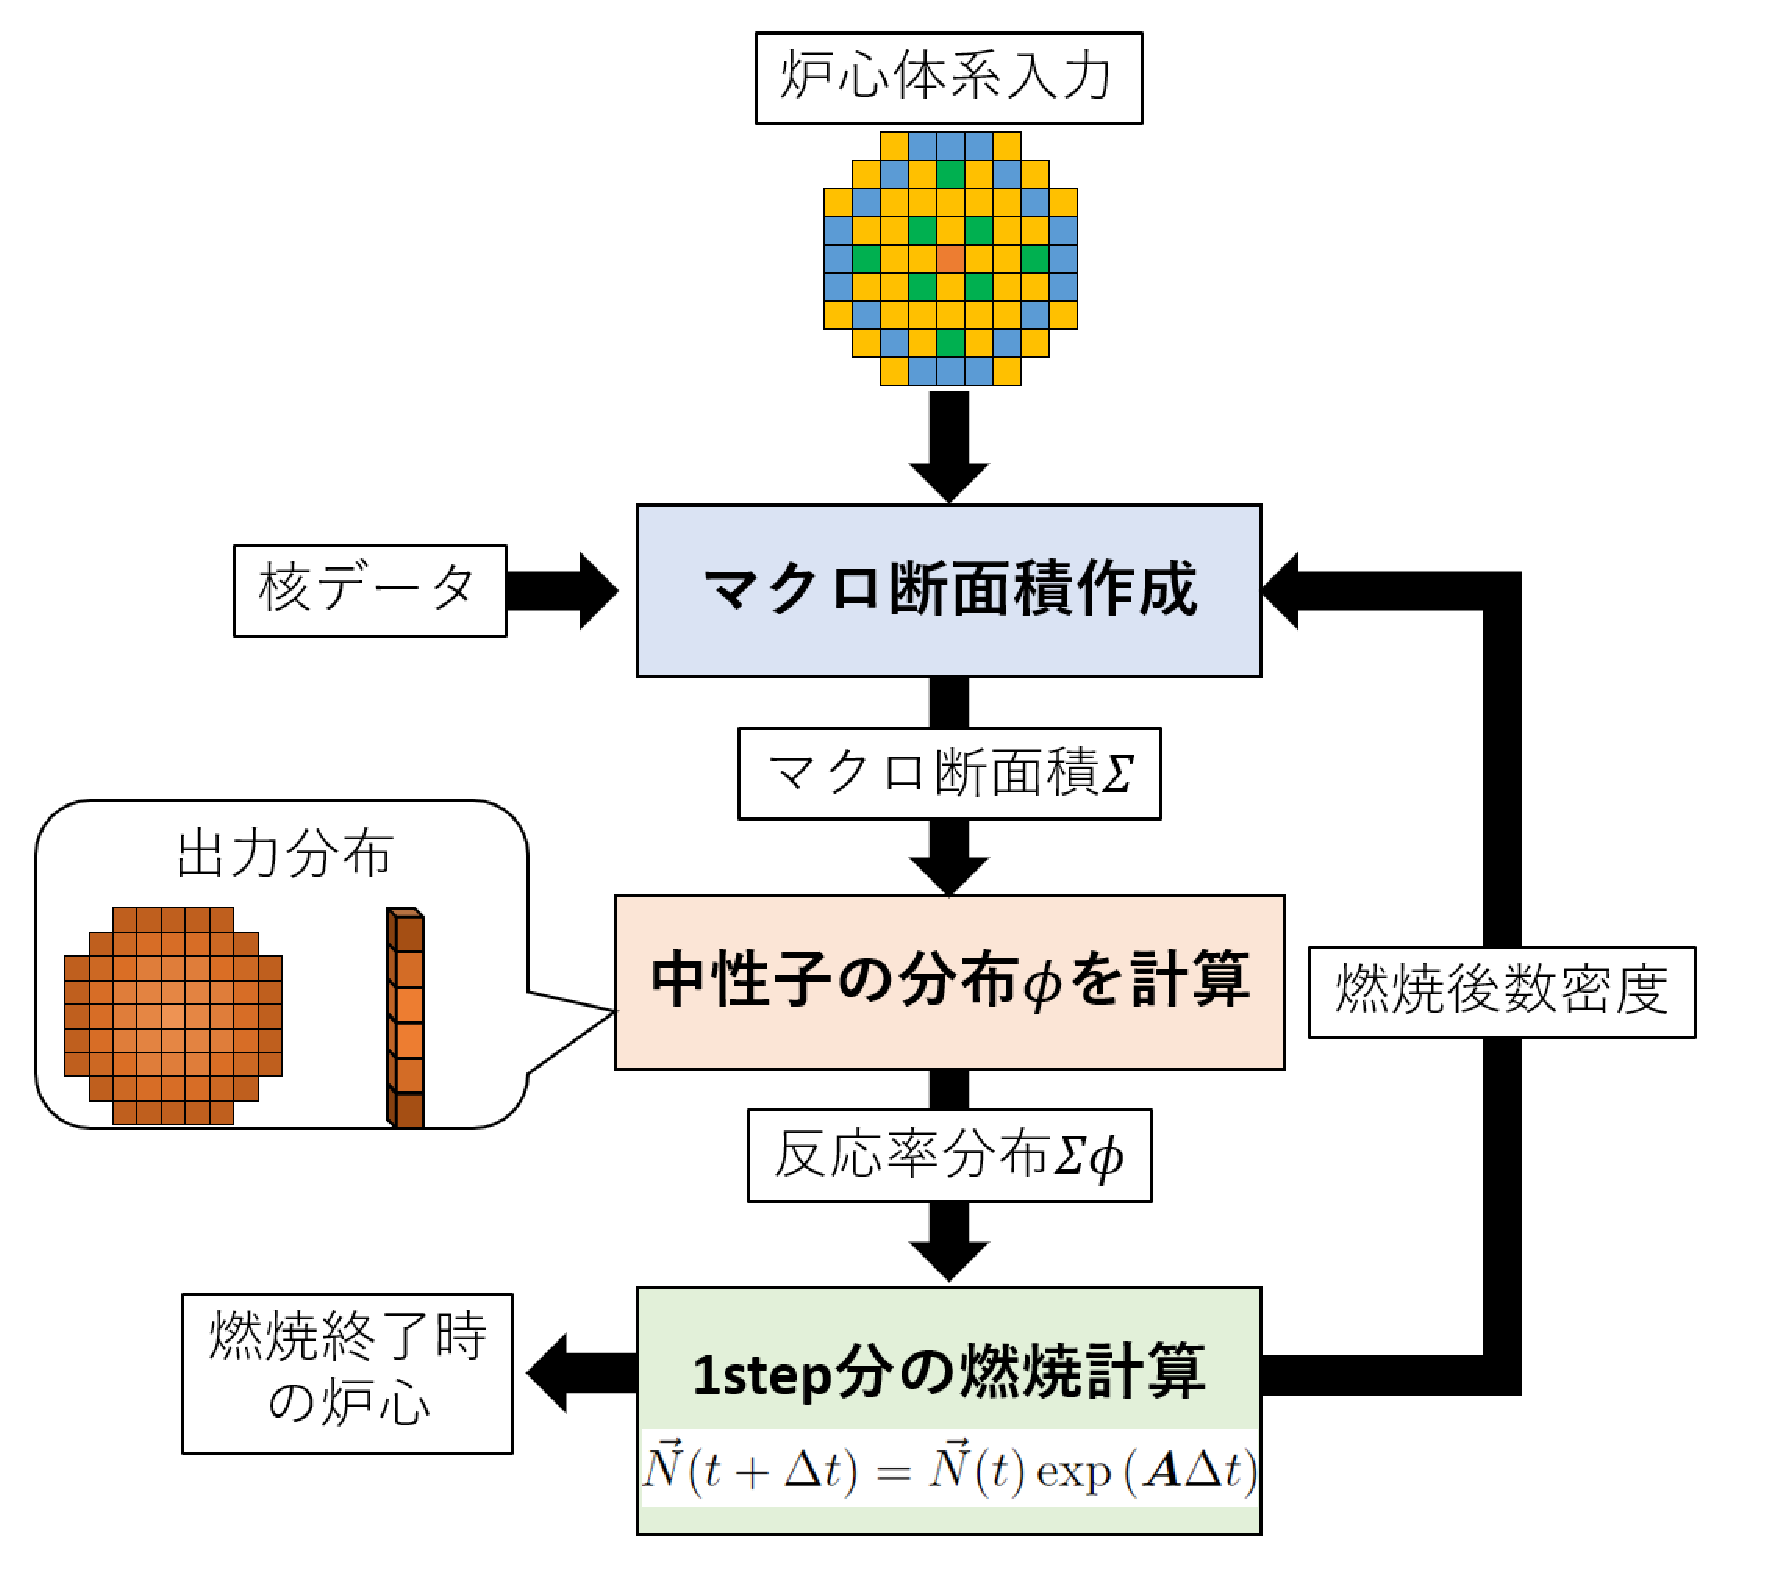
\includegraphics[width=120mm]{figure/time-discretization.eps}
  \caption{燃焼サイクルの時間的離散化}\label{time-discretization}
  \end{center}
\end{figure}

\begin{align}
  \Delta\vec{N} = \bm{A} \vec{N} \Delta t   \label{BurnupEqDis}
\end{align}
\begin{align}
  \vec{N}(t + \Delta t) = \vec{N}(t) \exp{( \bm{A} \Delta t )} \label{BurnupEqDisSol}
\end{align}


% 章ごとの参考文献欄
\printbibliography[segment=\therefsegment,heading=subbibliography]

\newpage